
%----------------------------------------------------------------------------------------
%	CHAPTER 3
%----------------------------------------------------------------------------------------
%Acronimos
\acrodef{RPC}{Remote Procedure Calls (LLamadas a Prodecimientos Remotos)}
\acrodef{SOA}{Service-oriented Architecture (Arquitectura basada en servicios)}
\acrodef{REST}{(Representation State Transfer) (Transferencia de Estado Representacional)}

\chapterimage{dibujo} % Chapter heading image

\chapter{Especificaciones t�cnicas }\label{chapter_3}
\subsection{Estudio del arte}
\pichskip{2em}
\parpic[r][t]{%
	\begin{minipage}{40mm}
		
\includegraphics[width=\linewidth]{logos/anny}%
	\end{minipage}
}
\subsubsection{Annyang-master}
Annyang-master \cite{Annyang} es una librer�a JavaScript con licencia MIT. Permite la interacci�n con el navegador Google Chrome mediante comandos de voz. Para el resto de navegadores no est� disponible. Es sencilla de utilizar y de incorporar a la web, tiene poco tama�o: 2KBytes.

\parpic[r][t]{%
	\begin{minipage}{40mm}
		
\includegraphics[width=\linewidth]{logos/ispeech}%
	\end{minipage}
}
{ \subsubsection{ISpeech API}}

El API iSpeech \cite{iSpeech} permite implementar \textit{Text-To-Speech} (TTS) y Automatizaci�n de Reconocimiento de Voz (ASR) en cualquier aplicaci�n con conexi�n a Internet. Las APIs son independientes de la plataforma lo que significa que cualquier dispositivo que pueda grabar o reproducir audio y est� conectado a Internet puede utilizar la API de iSpeech. Es necesario pagar para hacer uso de ella, la cantidad monetaria depende del n�mero de palabras que se deseen utilizar. Se encuentra disponible para BlackBerry, IPhone, Android y los navegadores web (estos mediante el SDK de .NET C\#, Java y PHP). Est� disponible en varios idiomas, entre ellos el espa�ol, ingl�s y chino.

\begin{minipage}{\textwidth}
\lstinputlisting[label=diccionario, caption={Fragmento del diccionario.}]{codigoFuente/tfg/diccionario.txt}
\end{minipage}


\subsubsection{Conexi�n desde el cliente web}
Para la conexi�n desde el cliente web al \textit{socket} que se ha creado en el servidor son necesarias dos cosas:
\begin{enumerate}
	\item A�adir la librer�a socket.io.js con la misma versi�n que el que se est� ejecutando en el servidor.
	\item Conectarse al socket mediante io.connect("http://localhost:3000").
\end{enumerate}
Tras estos dos pasos, el forma de utilizar el objeto \textit{socket} creado es similar a la vista en el servidor. El m�todo \textit{on} para recibir y el m�todo \textit{emit} para enviar. La soluci�n implementada en el TFG se puede ver en el Listado \ref{socketCliente}.
\lstinputlisting[label=socketCliente, caption=Socket en el cliente web,language=JavaScript]{codigoFuente/enia/socket.js.txt}


Adem�s en la figura \ref{grafica_rankingNavegadores} se puede ver la tendencia de cada uno de los navegadores \cite{RankingNavegador}.

\begin{figure}[h]
	\centering
	\begin{tikzpicture}
	
	\begin{axis}[
	/pgf/number format/.cd,
	use comma,
	1000 sep={},
	width=14cm, height=8cm,     % size of the image
	grid = major,
	grid style={dashed, gray!30},
	%xmode=log,log basis x=10,
	%ymode=log,log basis y=10,
	xmin=2010,     % start the diagram at this x-coordinate
	xmax=2015.4,    % end   the diagram at this x-coordinate
	ymin=0,     % start the diagram at this y-coordinate
	ymax=100,   % end   the diagram at this y-coordinate
	/pgfplots/xtick={2010,2011,...,2015}, % make steps of length 1
	/pgfplots/ytick={0,10,...,100}, % make steps of length 5
	axis background/.style={fill=white},
	ylabel= \% de uso,
	xlabel=A�o,
	tick align=outside,
	legend pos= north west]
	
	% Chrome
	\addplot coordinates {
		(2010,11)
		(2010.08,12)
		(2010.16,12)
		(2010.24,14)
		(2010.32,15)
		(2010.40,16)
		(2010.48,17)
		(2010.56,17)
		(2010.64,17)
		(2010.72,19)
		(2010.80,20)
		(2010.88,22)
		(2011,23)
		(2011.08,24)
		(2011.16,25)
		(2011.24,26)
		(2011.32,26)
		(2011.40,28)
		(2011.48,29)
		(2011.56,30)
		(2011.64,30)
		(2011.72,32)
		(2011.80,33)
		(2011.88,34)
		(2012,35)
		(2012.08,36)
		(2012.16,37)
		(2012.24,38)
		(2012.32,39)
		(2012.40,42)
		(2012.48,43)
		(2012.56,43)
		(2012.64,44)
		(2012.72,45)
		(2012.80,46)
		(2012.88,47)
		(2013,48)
		(2013.08,50)
		(2013.16,52)
		(2013.24,53)
		(2013.32,53)
		(2013.40,52)
		(2013.48,53)
		(2013.56,53)
		(2013.64,53)
		(2013.72,54)
		(2013.80,55)
		(2013.88,56)
		(2014,56)
		(2014.08,56)
		(2014.16,57)
		(2014.24,58)
		(2014.32,59)
		(2014.40,59)
		(2014.48,60)
		(2014.56,60)
		(2014.64,60)
		(2014.72,60)
		(2014.80,60)
		(2014.88,61)
		(2015,62)
		(2015.08,62)
		(2015.16,62)
		(2015.24,64)
		(2015.32,64)
		
		
	};
	\addlegendentry{Google Chrome}
	
	% IE
	\addplot coordinates {
		(2010,36)
		(2010.08,35)
		(2010.16,35)
		(2010.24,33)
		(2010.32,32)
		(2010.40,31)
		(2010.48,30)
		(2010.56,31)
		(2010.64,31)
		(2010.72,30)
		(2010.80,29)
		(2010.88,27)
		(2011,27)
		(2011.08,27)
		(2011.16,27)
		(2011.24,26)
		(2011.32,24)
		(2011.40,25)
		(2011.48,23)
		(2011.56,22)
		(2011.64,24)
		(2011.72,23)
		(2011.80,22)
		(2011.88,21)
		(2012,20)
		(2012.08,20)
		(2012.16,19)
		(2012.24,19)
		(2012.32,18)
		(2012.40,18)
		(2012.48,17)
		(2012.56,16)
		(2012.64,16)
		(2012.72,16)
		(2012.80,16)
		(2012.88,15)
		(2013,15)
		(2013.08,14)
		(2013.16,13)
		(2013.24,13)
		(2013.32,13)
		(2013.40,12)
		(2013.48,12)
		(2013.56,12)
		(2013.64,12)
		(2013.72,12)
		(2013.80,12)
		(2013.88,11)
		(2014,10)
		(2014.08,10)
		(2014.16,10)
		(2014.24,10)
		(2014.32,9)
		(2014.40,9)
		(2014.48,8)
		(2014.56,8)
		(2014.64,10)
		(2014.72,10)
		(2014.80,10)
		(2014.88,10)
		(2015,8)
		(2015.08,8)
		(2015.16,8)
		(2015.24,8)
		(2015.32,8)
		
		
	};
	\addlegendentry{Internet Explorer}
	
	% Mozilla Firefox
	\addplot coordinates {
		(2010,46)
		(2010.08,46)
		(2010.16,46)
		(2010.24,46)
		(2010.32,47)
		(2010.40,46)
		(2010.48,46)
		(2010.56,46)
		(2010.64,45)
		(2010.72,44)
		(2010.80,44)
		(2010.88,44)
		(2011,43)
		(2011.08,42)
		(2011.16,42)
		(2011.24,43)
		(2011.32,42)
		(2011.40,42)
		(2011.48,42)
		(2011.56,41)
		(2011.64,40)
		(2011.72,39)
		(2011.80,38)
		(2011.88,38)
		(2012,37)
		(2012.08,37)
		(2012.16,37)
		(2012.24,36)
		(2012.32,35)
		(2012.40,34)
		(2012.48,34)
		(2012.56,33)
		(2012.64,32)
		(2012.72,32)
		(2012.80,31)
		(2012.88,31)
		(2013,30)
		(2013.08,30)
		(2013.16,29)
		(2013.24,28)
		(2013.32,28)
		(2013.40,29)
		(2013.48,29)
		(2013.56,28)
		(2013.64,28)
		(2013.72,27)
		(2013.80,27)
		(2013.88,27)
		(2014,27)
		(2014.08,26)
		(2014.16,26)
		(2014.24,25)
		(2014.32,25)
		(2014.40,25)
		(2014.48,25)
		(2014.56,25)
		(2014.64,24)
		(2014.72,23)
		(2014.80,23)
		(2014.88,24)
		(2015,23)
		(2015.08,23)
		(2015.16,22)
		(2015.24,21)
		(2015.32,21)
		
		
	};
	\addlegendentry{Mozilla Firefox}
	
	% Safari
	\addplot coordinates {
		(2010,4)
		(2010.08,4)
		(2010.16,4)
		(2010.24,4)
		(2010.32,3)
		(2010.40,4)
		(2010.48,3)
		(2010.56,3)
		(2010.64,4)
		(2010.72,4)
		(2010.80,4)
		(2010.88,4)
		(2011,4)
		(2011.08,4)
		(2011.16,4)
		(2011.24,4)
		(2011.32,4)
		(2011.40,4)
		(2011.48,4)
		(2011.56,4)
		(2011.64,4)
		(2011.72,4)
		(2011.80,4)
		(2011.88,4)
		(2012,4)
		(2012.08,4)
		(2012.16,4)
		(2012.24,4)
		(2012.32,4)
		(2012.40,4)
		(2012.48,4)
		(2012.56,4)
		(2012.64,4)
		(2012.72,4)
		(2012.80,4)
		(2012.88,4)
		(2013,4)
		(2013.08,4)
		(2013.16,4)
		(2013.24,4)
		(2013.32,4)
		(2013.40,4)
		(2013.48,4)
		(2013.56,4)
		(2013.64,4)
		(2013.72,4)
		(2013.80,4)
		(2013.88,4)
		(2014,4)
		(2014.08,4)
		(2014.16,4)
		(2014.24,4)
		(2014.32,4)
		(2014.40,4)
		(2014.48,4)
		(2014.56,4)
		(2014.64,4)
		(2014.72,4)
		(2014.80,4)
		(2014.88,4)
		(2015,4)
		(2015.08,4)
		(2015.16,4)
		(2015.24,4)
		(2015.32,4)
		
	};
	\addlegendentry{Safari}
	
	% Opera
	\addplot coordinates {
		(2010,2)
		(2010.08,2)
		(2010.16,2)
		(2010.24,2)
		(2010.32,2)
		(2010.40,2)
		(2010.48,2)
		(2010.56,2)
		(2010.64,2)
		(2010.72,2)
		(2010.80,2)
		(2010.88,2)
		(2011,3)
		(2011.08,3)
		(2011.16,3)
		(2011.24,3)
		(2011.32,2)
		(2011.40,2)
		(2011.48,2)
		(2011.56,2)
		(2011.64,2)
		(2011.72,2)
		(2011.80,2)
		(2011.88,3)
		(2012,2)
		(2012.08,2)
		(2012.16,2)
		(2012.24,2)
		(2012.32,2)
		(2012.40,2)
		(2012.48,2)
		(2012.56,2)
		(2012.64,2)
		(2012.72,2)
		(2012.80,2)
		(2012.88,2)
		(2013,2)
		(2013.08,2)
		(2013.16,2)
		(2013.24,2)
		(2013.32,2)
		(2013.40,2)
		(2013.48,2)
		(2013.56,2)
		(2013.64,2)
		(2013.72,2)
		(2013.80,2)
		(2013.88,2)
		(2014,2)
		(2014.08,2)
		(2014.16,2)
		(2014.24,2)
		(2014.32,2)
		(2014.40,2)
		(2014.48,2)
		(2014.56,2)
		(2014.64,2)
		(2014.72,2)
		(2014.80,2)
		(2014.88,2)
		(2015,2)
		(2015.08,2)
		(2015.16,2)
		(2015.24,2)
		(2015.32,2)
		
		
	};
	\addlegendentry{Opera}
	
	\end{axis} 
	
	\end{tikzpicture}
	
	\caption{ Uso de los navegadores web \cite{RankingNavegador}.}
	\label{grafica_rankingNavegadores}
\end{figure}
\subsubsection{Subir/Bajar secci�n/subsecci�n}


\begin{figure}[!htb]
	\centering
	\begin{minipage}{0.49\textwidth}
		\centering
		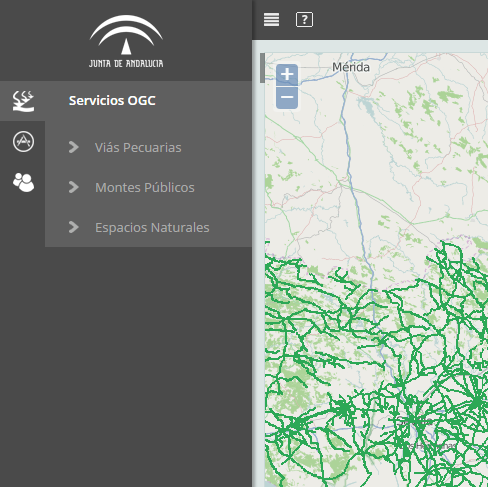
\includegraphics[width=\textwidth]{enia/seccion}
		\caption{Secci�n seleccionada.}
		\label{img_eniaSeccion}
	\end{minipage}
	~
	\begin{minipage}{0.49\textwidth}
		\centering
		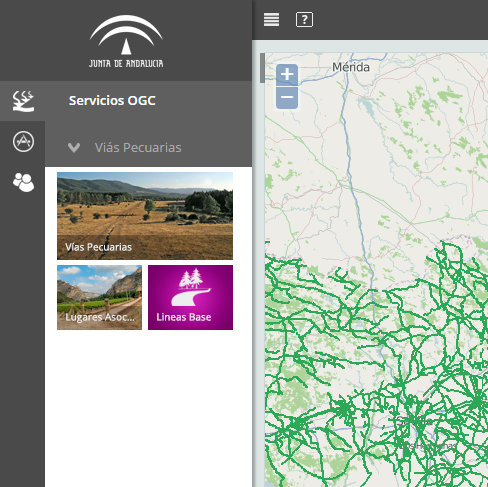
\includegraphics[width=\textwidth]{enia/subseccion}
		\caption{Subsecci�n seleccionada.}
		\label{img_eniaSubseccion}
	\end{minipage}
	
\end{figure}

